\chapter{Mobile phone screen content recognition module}
\label{ch:screen_recognize}
Mobile phone screen contains much of elements, but can be classified in two group: text and graphical element.
Understanding the meaning of phone screen requires to detect and recognize these elements.
In this chapter, basic objects in screen such as button, text and keyboard are covered.

\section{Technique using for detection}
\subsection{Edge detection}
\subsubsection{\gls{ced}}
The main purpose of edge detection is to obtain structure properties of the image with least data extracted for further image processing \cite{canny}. Among some algorithms existing, I choose the one developed by John F. Canny (JFC) \nocite{jfc_canny}. Known as Canny Edge detector or optimal detector, Canny algorithm has three main advantages \cite{code_canny}:
	\begin{itemize}
		\item \textbf{Low error rate}: Meaning a good detection of only existent edges.
		\item \textbf{Good localization}: The distance between edge pixels detected and real edge pixels have to be minimized.
		\item \textbf{Minimal response}: Only one detector response per edge.
	\end{itemize}

\subsubsection{CED algorithm steps}
\label{sec:ced_step}
\begin{enumerate}
	\item \textbf{Noise filter}: Using Gaussian filter \nocite{gauss_filter}, a sample kernel of \textit{size = 5} might be shown as Equation \ref{eq:gauss}:
	\begin{equation}
		\label{eq:gauss}
		B = \frac{1}{159} .
		\left[ \begin{array}{ccccc}
		2 & 4 & 5 & 4 & 2 \\
		5 & 12 & 15 & 12 & 5 \\
		4 & 9 & 12 & 9 & 4 \\
		2 & 4 & 5 & 4 & 2
		\end{array} \right]
	\end{equation}

	\item \textbf{Find the intensity gradient of the image}: Gradients at each pixel in the smoothed image are determined by applying Sobel-operator \cite{sobel_alg}:

	Apply a pair of convolution masks (in \textit{x} and \textit{y} directions:
	\begin{equation}
		\label{eq:gx_gy}
		G_x =
		\left[ \begin{array}{ccc}
		-1 & 0 & 1 \\
		-2 & 0 & 2 \\
		-1 & 0 & 1
		\end{array} \right]
		\qquad
		G_y =
		\left[ \begin{array}{ccc}
		1 & 2 & 1 \\
		0 & 0 & 0 \\
		-1 & -2 & -1
		\end{array} \right]
	\end{equation}

	Find the gradient strength and direction with:
	\begin{equation}
		\label{eq:gradient}
		G = \sqrt{G^2_x + G^2_y}
	\end{equation}
	\begin{equation}
		\label{eq:direction}
		\theta = arctan(\frac{G_y}{G_x})
	\end{equation}
	The direction is rounded to one of four possible angles (namely 0, 45, 90 or 135)

	\item \textbf{Apply Non-maximum suppression}: Removing pixels that are not considered to be part of an edge.
	\item \textbf{Double thresholding}: Potential edges are determined by thresholding.
	\item \textbf{Edge tracking by hysteresis}: Final edges are determined by suppressing all edges that are not connected to a very certain (strong) edge.
\end{enumerate}

\subsection{Shape detection}
\label{sec:shape_detect}
The output of CED process in Section \ref{sec:ced_step} is calculated to decide whether image contains simple geometric shapes (such as triangles, rectangles, squares, pentagons) or not.

For each edge, contour is retrieved for detecting process. Only contours with area greater than certain amount are considered. Practically, contours larger than 250 pixel are accepted.

Next, shape of the contour is decided by its attributes. For example, if the contour has 3 vertices, it is a triangle. Correspondingly, a contour has 4 vertices which all the angles in the contour are from 80 to 100 degree is a rectangle.

\subsection{Text detection and extraction}
\label{sec:text_detect}
Mobile phone screen is composed of much of text. Almost object in the screen has text with it. Text segmentation and recognition help the system to understanding the sense of the screen content.

Our system aims at the automatic detection of text. This is done by the algorithm. Figure \ref{fig:flow_diagram_morph} shows the flow diagram of text detection algorithm. The algorithm steps are summarized as follows.

\begin{enumerate}
	\item An Sobel edge detection scheme is applied to the gray scale image. The image I is blurred (to reduce false edges and over-segmentation) using open-close and close-open filters.
	The final blurred image Ib is the average of the outputs of these filters. The 3 x 3 8-connected structuring element of type ``square'' is used here.

	Next, the morphological gradient operator \nocite{morph} is applied to the blurred image Ib resulting in an image G as follows:
	\begin{center}
	G = Dilation (Ib) – Erosion (Ib)
	\end{center}

	The Morphological gradient is an edge-strength extraction operator that gives symmetric edges between foreground and background regions.

	The resulting image is then thresholded to obtain a binary edge image. Otsu and binary thresholding technique is used
	for that. \nocite{otsu}

	\item Closed edges in the binary edge image are grouped by dilation using eight- connected structuring elements.

	Then small connected components in the dilated image are filtered using erosion. The output is a binary image
	that contains text candidate regions.

	\item Connected component labeling is performed to label each object separately.

	\item After applying connected component labeling, the first set of criteria is applied which eliminate all objects whose area is greater than 10000 and filled area is greater than 8000.
	One more criteria namely major axis length is used which is used to retain the text region alone.
	All objects, whose major axis lengths are in between 20 to 3000, are considered to be text.
	To eliminate small objects, connected component labeling is applied to the resultant image and the second set of criteria is applied which eliminates all the objects whose area is less than 300 and filled area is less than 500.
\end{enumerate}

After applying all these 4 steps, we get a filtered image that contains only text regions \cite{text_detect}.

	\begin{figure}[H]
		\centering
		\includegraphics{Chapters/Fig/flow_diagram_morph.png}
		\caption{Flow diagram of Text Detection algorithm}
		\label{fig:flow_diagram_morph}
	\end{figure}

\subsection{Optical Character Recognition}
\label{sec:ocr}
By definition, \gls{ocr} is the process or technology of reading data in printed form by a device (optical character reader) that scans and identifies characters \cite{ocr_def}.

Tesseract is an open-source OCR engine having comparative recognition accuracy. Originally developed by HP between 1984 and 1994, Tesseract became open-source in 2005 and is developed by Google since 2006 \cite{ocr_overview}. According to 1995 UNLV results, Tesseract can achieve accuracy up to 98\% on English newspaper \cite{Rice_thefourth}.

Figure \ref{fig:tesseract_arch} briefly describes the architecture of Tesseract OCR engine \cite{tesseract_oscon}:

	\begin{figure}[H]
		\centering
		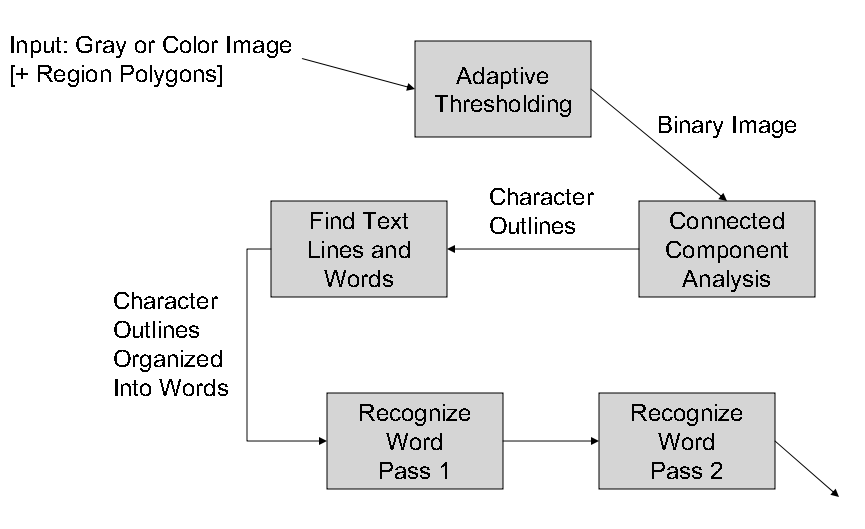
\includegraphics[scale=0.5]{Chapters/Fig/tesseract_arch.png}
		\caption{Tesseract OCR Architecture}
		\label{fig:tesseract_arch}
	\end{figure}

The output results of this phrase are used for naming objects which are identified in later script processing steps that we will discover in next chapter.

\section{Recognition result}
This section presents the result of unit testing for each image processing function of Image Processor component.

\subsection{Button detection}
Buttons are detected by shape using technique presented in Section \ref{sec:shape_detect}.

	\begin{figure}[H]
	    \centering
	    \subfigure{
	        \centering
	        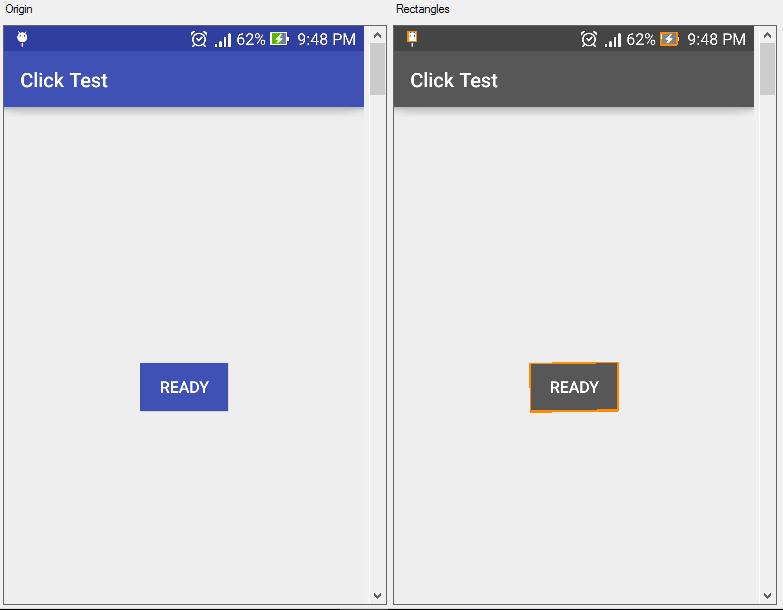
\includegraphics[scale=0.5]{Chapters/Fig/rect_detect.png}
	    }
	    
	    \subfigure{
	        \centering
	        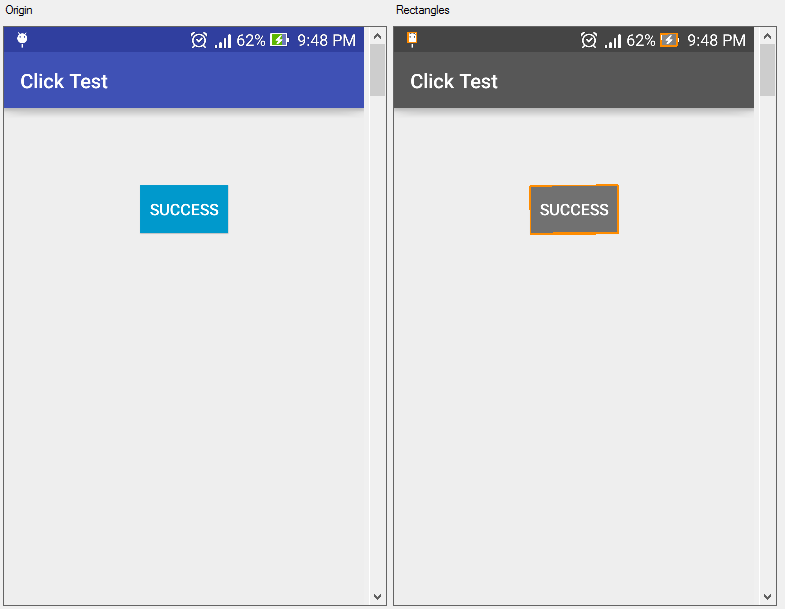
\includegraphics[scale=0.5]{Chapters/Fig/rect_detect_2.png}
	    }

	    \caption{Button detection result}
		\label{fig:btn_detect}
	\end{figure}

\subsection{Text detection}
Text is detected and segmented by algorithm in Section \ref{sec:text_detect}

	\begin{figure}[H]
	    \centering
	    \subfigure[Text detection in alarm home screen]{
	        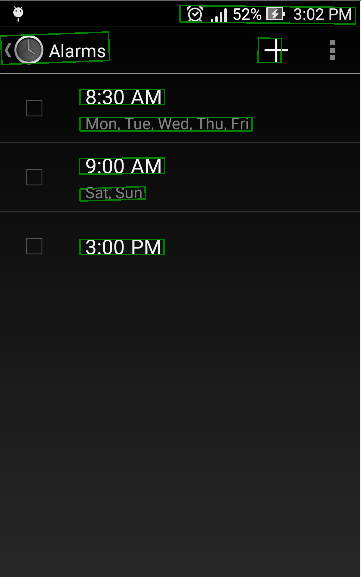
\includegraphics[scale=0.5]{Chapters/Fig/text_detect_home.png}
	    }
	    \qquad
	    \subfigure[Text detection in alarm item screen]{
	        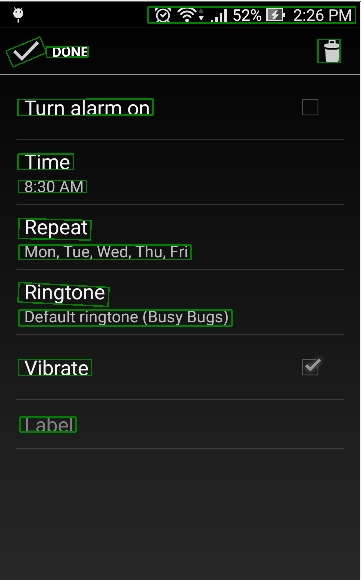
\includegraphics[scale=0.5]{Chapters/Fig/text_detect_item.png}
	    }
	    \qquad
	    \subfigure[Text detection in alarm time select screen]{
	        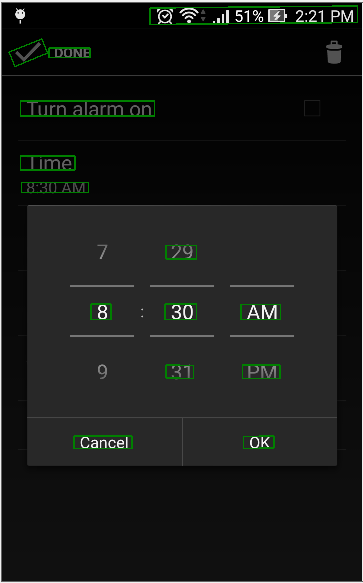
\includegraphics[scale=0.5]{Chapters/Fig/text_detect_clock.png}
	    }
	    \qquad
	    \caption{Text detection result}
		\label{fig:text_detect}
	\end{figure}

\subsection{Keyboard detection}
Keyboard consists of rectangle buttons. This feature shares the same detection method with Button detection.

	\begin{figure}[H]
		\centering
		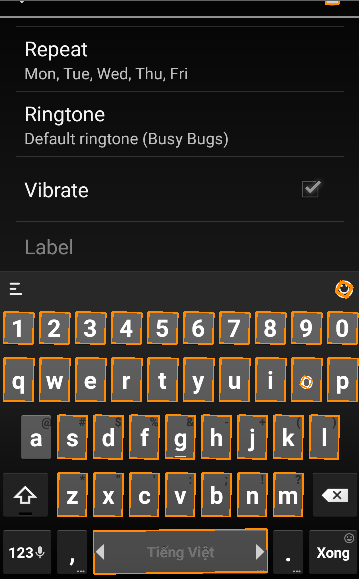
\includegraphics[scale=0.5]{Chapters/Fig/kb_detect.png}
		\caption{Keyboard detection result}
		\label{fig:kb_detect}
	\end{figure}

\subsection{Optical Character Recognition}
Text segments detected in previous section is used for recognizing process. After this stage, object will have a name given from recognized text and a relative location on the screen.

	\begin{figure}[H]
	    \centering
	    \subfigure[Text recognition in alarm home screen]{
	        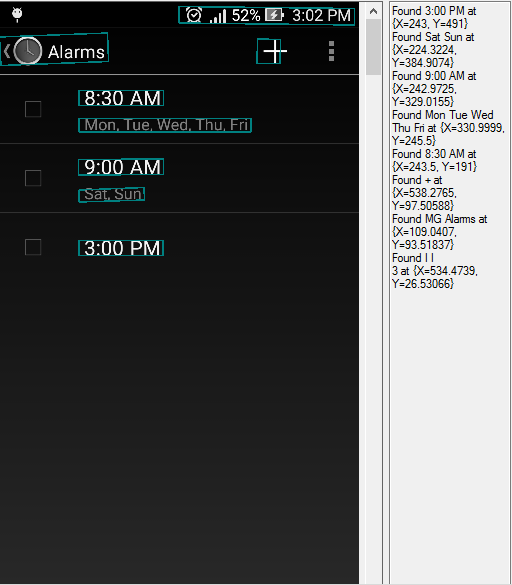
\includegraphics[scale=0.5]{Chapters/Fig/found_home.png}
	    }
	    \qquad
	    \subfigure[Text recognition in alarm item screen]{
	        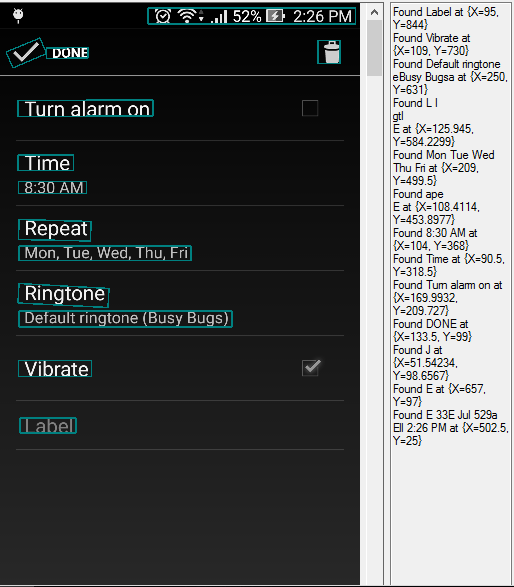
\includegraphics[scale=0.5]{Chapters/Fig/found_item.png}
	    }
	    \qquad
	    \subfigure[Text recognition in alarm time select screen]{
	        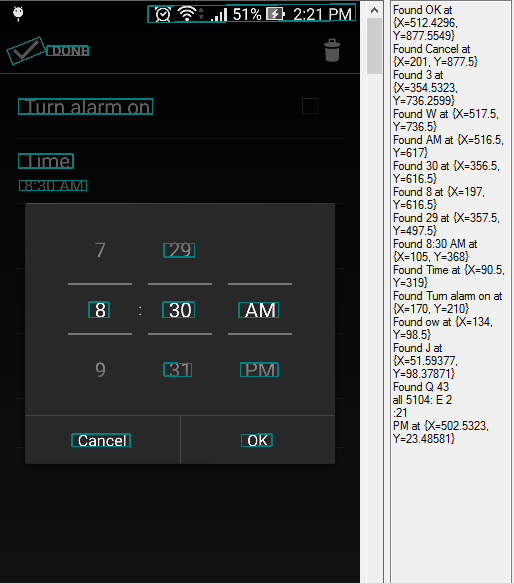
\includegraphics[scale=0.5]{Chapters/Fig/found_clock.png}
	    }
	    \qquad
	    \caption{Text recognition result}
		\label{fig:text_recognize}
	\end{figure}
